%-------------------------------------------------------------------------------
\chapter{Comparing the Pruning Strategies}
\labelchapter{app.quick}

%-------------------------------------------------------------------------------
This Appendix provides further data on the empirical \myLongAc{QoS}{Quality of Service} estimations that were introduced in Section \ref{ch.expe:sec.qece:ssec.impl}.
It shows the impact of the different pruning strategies for partitioning a given design space, with a particular focus on the quick pruning strategy that was defined in Algorithm \ref{ch.dse:sec.functional:ssec.basic:algo.quick}. 
For an easier representation of the results, we fix the {\it vector width} parameter to 8, as was done in Section \ref{ch.expe:sec.estimators:ssec.qos}.

In a similar way to what was done in Table \ref{ch.expe:sec.strategies:ssec.qos:table.quick}, we consider 4 different strategies for these experiments:
\begin{itemize}
    \item {\bf Strategy 1:} exhaustive pruning
    \item {\bf Strategy 2:} exhaustive pruning, with space reduction
    \item {\bf Strategy 3:} quick pruning, with space reduction (using \lstinline{SeqSpace})
    \item {\bf Strategy 4:} quick pruning, with space reduction (using \lstinline{MatrixSpace})
\end{itemize}

\vspace*{\fill}
\minilof

\clearpage

Table \ref{app.quick:table.strategies} introduces 8 different experiments for comparing those strategies --- see Table \ref{ch.expe:sec.strategies:ssec.qos:table.quick} for a detailed explanation of these experiments --- along with heat map representations of the \myAc{QoS} evolution.
For those experiments, we set the acceptable error threshold to 1\%, similarly to what was done in Figure \ref{ch.expe:sec.strategies:ssec.qos:fig.quick}.

As can be observed, the speed of the exhaustive strategies does not seem to be correlated with the initial distribution or with the number of simulations.
In fact, it seems that each simulation runtime is negligible with respect to the static cost of launching the simulator, resulting in a null gain when reducing the number of simulations.
However, as {\bf dot products} are quite simple kernels, it is possible that for more complex ones, the simulation runtime would scale, meaning that reducing the number of simulations could bring better performance.

On the other hand, we remark that changing the distribution (\ie the simulation workload) can have a direct impact on the number of implementations that are explored to build the {\bf pruning frontier}, thus impacting the duration of each strategy --- as the pruned space width reduces, it is easier to build that frontier and thus the pruning process becomes faster.
Moreover, we can use those results to confirm the impact that the space structures have on the exploration runtime.
We can remark that using a linear \lstinline{SeqSpace} can be more time-consuming than an exhaustive exploration of the space, while using a more complex \lstinline{MatrixSpace} implementation can result in an acceleration factor of $\times 5.4$, depending on the size of the pruned search space.

Finally, we can state that reducing the number of dimensions before the exploration is indeed an easy way to reduce the search time, under the assumtion that the user is aware that a particular dimension has no impact on a given metric for the considered exploration step.

As a conclusion, we can state that for \myAc{QoS}-based pruning, it seems to be better to use the {\bf quick pruning strategy} with a \lstinline{MatrixSpace} {\bf structure}, after performing {\bf space reduction}.\footnote{Here, only the {\it parallelism} dimension is being ignored at simulation time as it does not impact the implementations \myAc{QoS}. Moreover, as the {\it vector width} is fixed to 8, the exploration is thus in fact done in a {\bf two dimensional} space.}
One should also adapt the number of simulations in order to cope with the {\bf law of large numbers} and provide meaningful \myAc{QoS} results.

\clearpage

\begin{sidewaystable}[h!]
    \begin{tabular}{|c|cc|c|cc|cc|cc|cc|}
        \hline
        \multirow{2}*{{\bf \#}} & \multicolumn{2}{c|}{{\bf Distribution}} & {\bf Simulation} & \multicolumn{2}{|c|}{{\bf Strategy 1}} & \multicolumn{2}{|c|}{{\bf Strategy 2}} & \multicolumn{2}{|c|}{{\bf Strategy 3}} & \multicolumn{2}{c|}{{\bf Strategy 4}}\\
        ~ & Mean & Std dev. & {\bf number} & \#impl. & Time & \#impl. & Time & \#impl. & Time & \#impl. & Time\\
        \hline
        \ref{app.quick:fig.qos0-1-10} & 0 & 1 & 10 & 3844 & 12m26s & 961 & 3m08s & 275 & 5m23s & 275 & 54s\\ 
        \ccg \ref{app.quick:fig.qos0-1-50} & \ccg 0 &\ccg 1 & \ccg 50 & \ccg 3844 & \ccg 12m24s & \ccg 961 & \ccg 3m08s & \ccg 270 & \ccg 5m17s & \ccg 270 & \ccg 52s\\
        \ref{app.quick:fig.qos0-1-100} & 0 & 1 & 100 & 3844 & 12m22s & 961 & 3m09s & 260 & 5m06s & 260 & 49s\\
        \ccg \ref{app.quick:fig.qos0-1-1000} & \ccg 0 & \ccg 1 & \ccg 1000 & \ccg 3844 & \ccg 12m22s & \ccg 961 & \ccg 3m07s & \ccg 255 & \ccg 5m03s & \ccg 255 & \ccg 49s\\ 
        \ref{app.quick:fig.qos32-10-10} & 32 & 10 & 10 & 3844 & 12m24s & 961 & 3m09s & 181 & 3m23s & 181 & 35s\\ 
        \ccg \ref{app.quick:fig.qos32-10-50} & \ccg 32 &\ccg 10 & \ccg 50 & \ccg 3844 & \ccg 12m25s & \ccg 961 & \ccg 3m06s & \ccg 181 & \ccg 3m23s & \ccg 181 & \ccg 35s\\
        \ref{app.quick:fig.qos32-10-100} & 32 & 10 & 100 & 3844 & 12m32s & 961 & 3m08s & 181 & 3m24ss & 181 & 35s\\
        \ccg \ref{app.quick:fig.qos32-10-1000} & \ccg 32 & \ccg 10 & \ccg 1000 & \ccg 3844 & \ccg 12m20s & \ccg 961 & \ccg 3m07s & \ccg 181 & \ccg 3m25s & \ccg 181 & \ccg 35s\\ 
        \hline
    \end{tabular}
    \caption[Comparison of the pruning strategies on dot products]{Comparison of the pruning strategies on dot product implementations}
    \label{app.quick:table.strategies}
\end{sidewaystable}

\clearpage

\begin{figure}
    \centering
    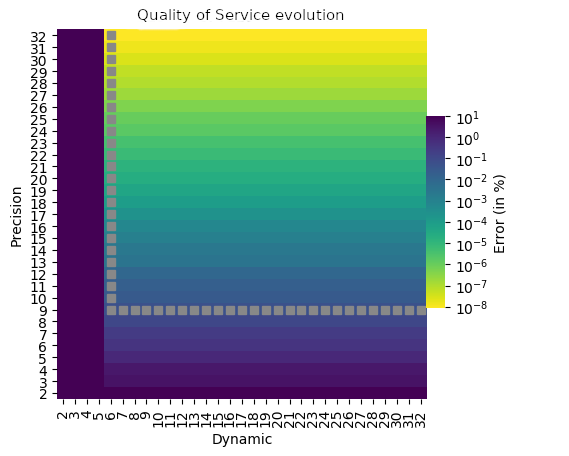
\includegraphics[width=.8\textwidth]{Figures/results/d2-32_p2-32_e8-8_N0-1_s10-0.png}
    \caption{Quality of service evolution ($\mathcal{N}(0, 1)$, 10 simulations)}
    \label{app.quick:fig.qos0-1-10}
\end{figure}
\begin{figure}
    \centering
    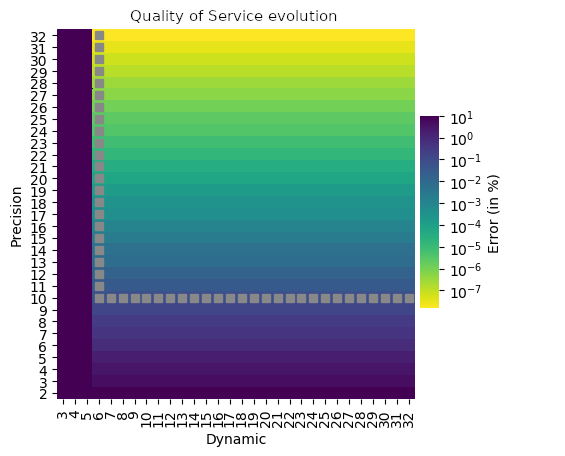
\includegraphics[width=.8\textwidth]{Figures/results/d2-32_p2-32_e8-8_N0-1_s50-0.png}
    \caption{Quality of service evolution ($\mathcal{N}(0, 1)$, 50 simulations)}
    \label{app.quick:fig.qos0-1-50}
\end{figure}
\begin{figure}
    \centering
    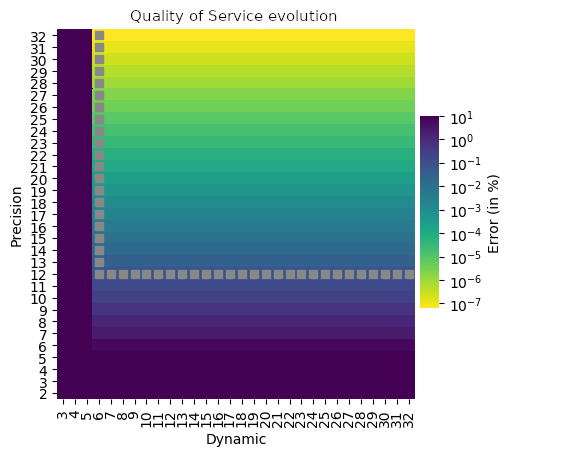
\includegraphics[width=.8\textwidth]{Figures/results/d2-32_p2-32_e8-8_N0-1_s100-0.png}
    \caption{Quality of service evolution ($\mathcal{N}(0, 1)$, 100 simulations)}
    \label{app.quick:fig.qos0-1-100}
\end{figure}
\begin{figure}
    \centering
    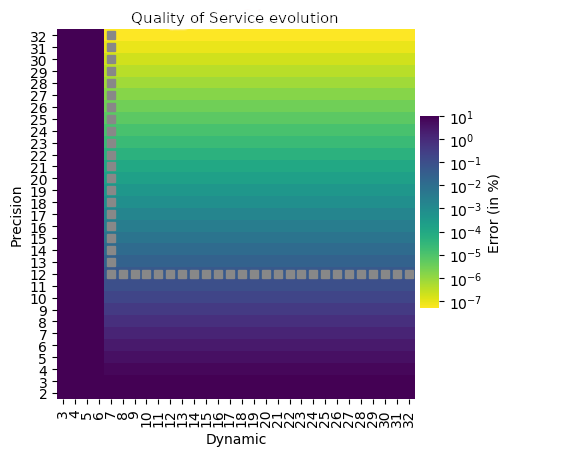
\includegraphics[width=.8\textwidth]{Figures/results/d2-32_p2-32_e8-8_N0-1_s1000-0.png}
    \caption{Quality of service evolution ($\mathcal{N}(0, 1)$, 1000 simulations)}
    \label{app.quick:fig.qos0-1-1000}
\end{figure}

\begin{figure}
    \centering
    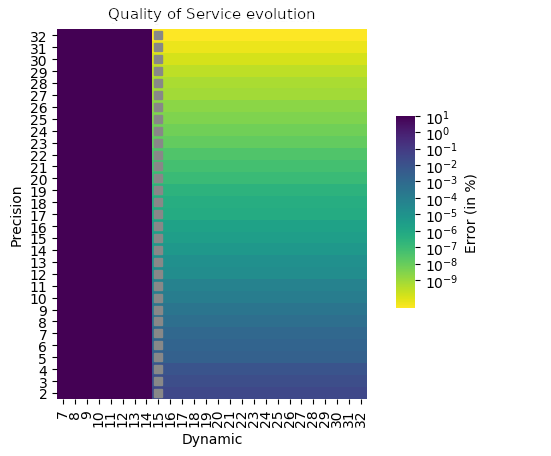
\includegraphics[width=.8\textwidth]{Figures/results/d2-32_p2-32_e8-8_N32-10_s10-0.png}
    \caption{Quality of service evolution ($\mathcal{N}(32, 10)$, 10 simulations)}
    \label{app.quick:fig.qos32-10-10}
\end{figure}
\begin{figure}
    \centering
    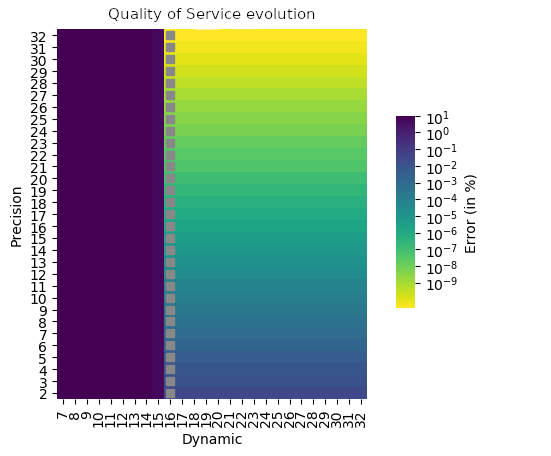
\includegraphics[width=.8\textwidth]{Figures/results/d2-32_p2-32_e8-8_N32-10_s50-0.png}
    \caption{Quality of service evolution ($\mathcal{N}(32, 10)$, 50 simulations)}
    \label{app.quick:fig.qos32-10-50}
\end{figure}
\begin{figure}
    \centering
    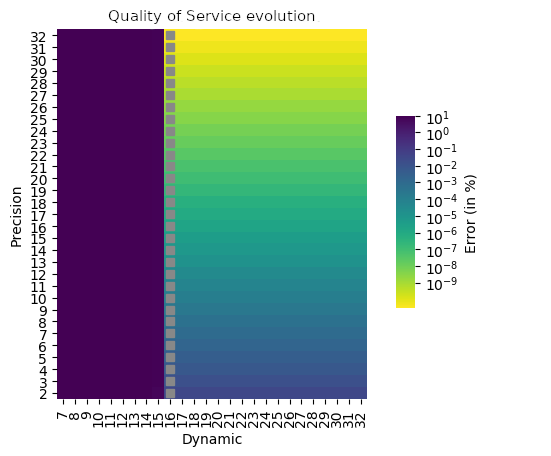
\includegraphics[width=.8\textwidth]{Figures/results/d2-32_p2-32_e8-8_N32-10_s100-0.png}
    \caption{Quality of service evolution ($\mathcal{N}(32, 10)$, 100 simulations)}
    \label{app.quick:fig.qos32-10-100}
\end{figure}
\begin{figure}
    \centering
    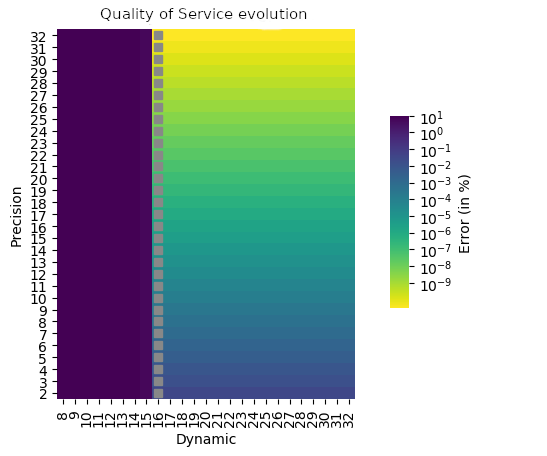
\includegraphics[width=.8\textwidth]{Figures/results/d2-32_p2-32_e8-8_N32-10_s1000-0.png}
    \caption{Quality of service evolution ($\mathcal{N}(32, 10)$, 1000 simulations)}
    \label{app.quick:fig.qos32-10-1000}
\end{figure}
